% answers.tex —— 2020 年·全国Ⅲ卷·文科 · 参考答案与详细解析片段
% 由 tools/generate_projects.py 依来源总账自 2020/2020_数学真题_全国3文_试题.md + 2020/2020_数学真题_全国3文_解析正文.md + 2020/2020_数学真题_全国3文_答案要点.md 生成，勿手改（改源 MD 后重跑）


\begin{answer}
\gksolhead{1}{}

\textbf{题目}：

已知集合 $A=\{1,2,3,5,7,11\}$，$B=\{x\mid 3<x<15\}$，则 $A\cap B$ 中元素的个数为\mbox{（　　）}
（A）$2$；（B）$3$；（C）$4$；（D）$5$。

\Needspace{4\baselineskip}
\textbf{解析}
\Needspace{5\baselineskip}
$B=\{x\mid 3<x<15\}$ 是开区间 $(3,15)$。逐个检验 $A$ 中的元素：$1$，$2$，$3$ 都不满足 $3<x<15$，而
\nopagebreak[4]
\[5\in(3,15),\qquad 7\in(3,15),\qquad 11\in(3,15),\]
\Needspace{5\baselineskip}
故
\nopagebreak[4]
\[A\cap B=\{5,7,11\},\]
元素个数为 $3$。
选 B。

\gkanswer{答案：B。$A$ 中满足 $3<x<15$ 的元素为 $5$，$7$，$11$，共 $3$ 个，即 $A\cap B=\{5,7,11\}$。}

\end{answer}
\begin{answer}
\gksolhead{2}{}

\textbf{题目}：

若 $\bar z(1+\mathrm i)=1-\mathrm i$，则 $z=$\mbox{（　　）}
（A）$1-\mathrm i$；（B）$1+\mathrm i$；（C）$-\mathrm i$；（D）$\mathrm i$。

\Needspace{4\baselineskip}
\textbf{解析}
\Needspace{5\baselineskip}
记 $w=\bar z$，由 $w(1+\mathrm i)=1-\mathrm i$ 得
\nopagebreak[4]
\[w=\frac{1-\mathrm i}{1+\mathrm i}=\frac{(1-\mathrm i)^2}{(1+\mathrm i)(1-\mathrm i)}=\frac{1-2\mathrm i+\mathrm i^2}{1-\mathrm i^2}=\frac{-2\mathrm i}{2}=-\mathrm i .\]
\Needspace{5\baselineskip}
所以 $\bar z=-\mathrm i$，两边取共轭得
\nopagebreak[4]
\[z=\mathrm i .\]
代回验证：$\bar z(1+\mathrm i)=(-\mathrm i)(1+\mathrm i)=-\mathrm i-\mathrm i^2=1-\mathrm i$，相符。
选 D。

\gkanswer{答案：D。$\bar z=\dfrac{1-\mathrm i}{1+\mathrm i}=-\mathrm i$，故 $z=\mathrm i$。}

\end{answer}
\begin{answer}
\gksolhead{3}{}

\textbf{题目}：

设一组样本数据 $x_1,x_2,\cdots,x_n$ 的方差为 $0.01$，则数据 $10x_1,10x_2,\cdots,10x_n$ 的方差为\mbox{（　　）}
（A）$0.01$；（B）$0.1$；（C）$1$；（D）$10$。

\Needspace{4\baselineskip}
\textbf{解析}
\Needspace{5\baselineskip}
设原数据的平均数为 $\bar x$，由方差的定义
\nopagebreak[4]
\[s^2=\frac1n\sum_{i=1}^n(x_i-\bar x)^2=0.01 .\]
\Needspace{5\baselineskip}
新数据 $y_i=10x_i$ 的平均数为 $10\bar x$，故
\nopagebreak[4]
\[s'^2=\frac1n\sum_{i=1}^n(10x_i-10\bar x)^2=100\cdot\frac1n\sum_{i=1}^n(x_i-\bar x)^2=100\times0.01=1 .\]
即每个数据同乘 $10$ 时，方差乘 $10^2$。
选 C。

\gkanswer{答案：C。数据同乘 $10$，方差乘 $10^2$，即 $100\times0.01=1$。}

\end{answer}
\begin{answer}
\gksolhead{4}{}

\textbf{题目}：

Logistic 模型是常用数学模型之一，可应用于流行病学领域。有学者根据公布数据建立了某地区新冠肺炎累计确诊病例数 $I(t)$（$t$ 的单位：天）的 Logistic 模型：$I(t)=\dfrac K{1+\mathrm e^{-0.23(t-53)}}$，其中 $K$ 为最大确诊病例数。当 $I(t^*)=0.95K$ 时，标志着已初步遏制疫情，则 $t^*$ 约为（$\ln19\approx3$）\mbox{（　　）}
（A）$60$；（B）$63$；（C）$66$；（D）$69$。

\Needspace{4\baselineskip}
\textbf{解析}
\Needspace{5\baselineskip}
由 $I(t^*)=0.95K$ 得
\nopagebreak[4]
\[\frac K{1+\mathrm e^{-0.23(t^*-53)}}=0.95K\ \Longrightarrow\ 1+\mathrm e^{-0.23(t^*-53)}=\frac1{0.95}=\frac{20}{19},\]
\Needspace{5\baselineskip}
故
\nopagebreak[4]
\[\mathrm e^{-0.23(t^*-53)}=\frac1{19}\ \Longrightarrow\ -0.23(t^*-53)=-\ln19 .\]
\Needspace{5\baselineskip}
于是
\nopagebreak[4]
\[t^*=53+\frac{\ln19}{0.23}\approx53+\frac3{0.23}=53+13.04=66.04,\]
即 $t^*$ 约为 $66$。
选 C。

\gkanswer{答案：C。由 $\dfrac K{1+\mathrm e^{-0.23(t^*-53)}}=0.95K$ 得 $\mathrm e^{-0.23(t^*-53)}=\dfrac1{19}$，故 $t^*=53+\dfrac{\ln19}{0.23}\approx53+13=66$。}

\end{answer}
\begin{answer}
\gksolhead{5}{}

\textbf{题目}：

已知 $\sin\theta+\sin\left(\theta+\dfrac\pi3\right)=1$，则 $\sin\left(\theta+\dfrac\pi6\right)=$\mbox{（　　）}
（A）$\dfrac12$；（B）$\dfrac{\sqrt3}3$；（C）$\dfrac23$；（D）$\dfrac{\sqrt2}2$。

\Needspace{4\baselineskip}
\textbf{解析}
\Needspace{5\baselineskip}
用和角公式展开第二项：
\nopagebreak[4]
\[\sin\theta+\sin\left(\theta+\frac\pi3\right)=\sin\theta+\sin\theta\cos\frac\pi3+\cos\theta\sin\frac\pi3=\frac32\sin\theta+\frac{\sqrt3}2\cos\theta,\]
\Needspace{5\baselineskip}
故条件化为
\nopagebreak[4]
\[\frac32\sin\theta+\frac{\sqrt3}2\cos\theta=1 .\]
\Needspace{5\baselineskip}
而
\nopagebreak[4]
\[\sin\left(\theta+\frac\pi6\right)=\frac{\sqrt3}2\sin\theta+\frac12\cos\theta=\frac1{\sqrt3}\left(\frac32\sin\theta+\frac{\sqrt3}2\cos\theta\right)=\frac1{\sqrt3}\times1=\frac{\sqrt3}3 .\]
选 B。

\gkanswer{答案：B。条件化为 $\sqrt3\sin\theta+\cos\theta=\dfrac2{\sqrt3}$，而 $\sin\left(\theta+\dfrac\pi6\right)=\dfrac12\left(\sqrt3\sin\theta+\cos\theta\right)=\dfrac{\sqrt3}3$。}

\end{answer}
\begin{answer}
\gksolhead{6}{}

\textbf{题目}：

在平面内，$A$，$B$ 是两个定点，$C$ 是动点。若 $\overrightarrow{AC}\cdot\overrightarrow{BC}=1$，则点 $C$ 的轨迹为\mbox{（　　）}
（A）圆；（B）椭圆；（C）抛物线；（D）直线。

\Needspace{4\baselineskip}
\textbf{解析}
\Needspace{5\baselineskip}
以直线 $AB$ 为 $x$ 轴、$AB$ 的中点为原点建系，设
\nopagebreak[4]
\[A(-a,0),\qquad B(a,0)\quad(a>0),\qquad C(x,y).\]
\Needspace{5\baselineskip}
则
\nopagebreak[4]
\[\overrightarrow{AC}=(x+a,\ y),\qquad \overrightarrow{BC}=(x-a,\ y),\]
\Needspace{5\baselineskip}
由 $\overrightarrow{AC}\cdot\overrightarrow{BC}=1$ 得
\nopagebreak[4]
\[(x+a)(x-a)+y^2=1\ \Longrightarrow\ x^2+y^2=a^2+1 .\]
这是以 $AB$ 中点为圆心、$\sqrt{a^2+1}$ 为半径的圆（$a>0$ 时半径为正），故轨迹是圆。
选 A。

\gkanswer{答案：A。设 $A(-a,0)$，$B(a,0)$，$C(x,y)$，则 $(x+a)(x-a)+y^2=1$，即 $x^2+y^2=a^2+1$，轨迹是圆。}

\end{answer}
\begin{answer}
\gksolhead{7}{}

\textbf{题目}：

设 $O$ 为坐标原点，直线 $x=2$ 与抛物线 $C:y^2=2px$（$p>0$）交于 $D$，$E$ 两点。若 $OD\perp OE$，则 $C$ 的焦点坐标为\mbox{（　　）}
（A）$\left(\dfrac14,0\right)$；（B）$\left(\dfrac12,0\right)$；（C）$(1,0)$；（D）$(2,0)$。

\Needspace{4\baselineskip}
\textbf{解析}
\Needspace{5\baselineskip}
在 $x=2$ 上，$y^2=2p\cdot2=4p$，故可设
\nopagebreak[4]
\[D(2,2\sqrt p),\qquad E(2,-2\sqrt p).\]
\Needspace{5\baselineskip}
则
\nopagebreak[4]
\[\overrightarrow{OD}\cdot\overrightarrow{OE}=2\times2+2\sqrt p\times(-2\sqrt p)=4-4p .\]
\Needspace{5\baselineskip}
由 $OD\perp OE$ 得 $4-4p=0$，即 $p=1$。此时 $C:y^2=2x$，焦点为
\nopagebreak[4]
\[\left(\frac p2,0\right)=\left(\frac12,0\right).\]
选 B。

\gkanswer{答案：B。$D(2,2\sqrt p)$，$E(2,-2\sqrt p)$，由 $\overrightarrow{OD}\cdot\overrightarrow{OE}=4-4p=0$ 得 $p=1$，焦点为 $\left(\dfrac12,0\right)$。}

\end{answer}
\begin{answer}
\gksolhead{8}{}

\textbf{题目}：

点 $(0,-1)$ 到直线 $y=k(x+1)$ 距离的最大值为\mbox{（　　）}
（A）$1$；（B）$\sqrt2$；（C）$\sqrt3$；（D）$2$。

\Needspace{4\baselineskip}
\textbf{解析}
\Needspace{5\baselineskip}
直线 $y=k(x+1)$ 即 $kx-y+k=0$，点 $(0,-1)$ 到它的距离为
\nopagebreak[4]
\[d(k)=\frac{|k\cdot0-(-1)+k|}{\sqrt{k^2+1}}=\frac{|k+1|}{\sqrt{k^2+1}} .\]
\Needspace{5\baselineskip}
平方后比较：
\nopagebreak[4]
\[d^2=\frac{(k+1)^2}{k^2+1},\]
\Needspace{5\baselineskip}
而
\nopagebreak[4]
\[2(k^2+1)-(k+1)^2=k^2-2k+1=(k-1)^2\geqslant0,\]
故 $(k+1)^2\leqslant2(k^2+1)$，即 $d^2\leqslant2$，$d\leqslant\sqrt2$。当 $k=1$ 时等号成立，故最大值为 $\sqrt2$。
选 B。

\gkanswer{答案：B。距离 $d=\dfrac{|k+1|}{\sqrt{k^2+1}}$，由 $2(k^2+1)-(k+1)^2=(k-1)^2\geqslant0$ 得 $d\leqslant\sqrt2$，$k=1$ 时取等号。}

\end{answer}
\begin{answer}
\gksolhead{9}{}

\textbf{题目}：

下图为某几何体的三视图，则该几何体的表面积是\mbox{（　　）}
（A）$6+4\sqrt2$；（B）$4+4\sqrt2$；（C）$6+2\sqrt3$；（D）$4+2\sqrt3$。
\nopagebreak[4]
\begin{center}% 2020 全国Ⅲ卷 文9：某几何体的三视图
% 来源 PDF：普通高考/2020/2020全国3文(云南,广西,贵州,西藏,四川).pdf 第 1 页（A3 横排），印面 1127，第 9 题题干下方
% 结构（按原页 300 dpi 量取）：主视图、左视图、俯视图均为腰长 2 的等腰直角三角形；
%   主视图直角在右下，左视图直角在左下，俯视图直角在右上。三视图的直角互相对应，
%   故该几何体是三条两两垂直的棱长均为 2 的四面体。
% 尺寸标注：原页只在主视图底边、主视图右边、俯视图右边标出「2」，此处照录。
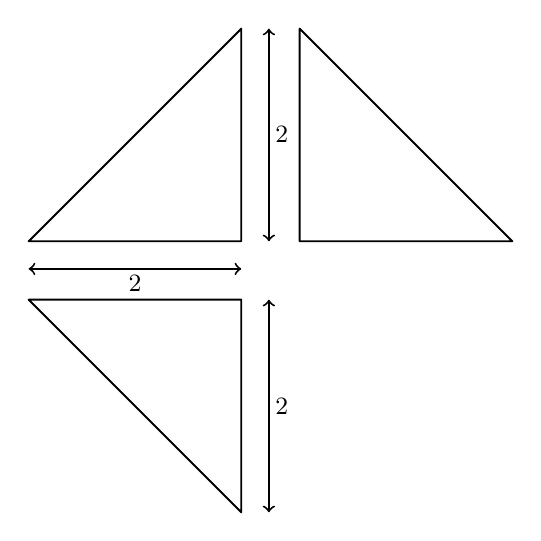
\begin{tikzpicture}[line width=0.7pt, font=\small,
  x=1.35cm, y=1.35cm, line cap=round, line join=round]

  % 主视图：直角边 2 与 2，直角在右下
  \draw (0,0) -- (2,0) -- (2,2) -- cycle;

  % 左视图：直角边 2 与 2，直角在左下
  \draw (2.55,0) -- (4.55,0) -- (2.55,2) -- cycle;

  % 俯视图：直角边 2 与 2，直角在右上
  \draw (0,-0.55) -- (2,-0.55) -- (2,-2.55) -- cycle;

  % 尺寸标注
  \draw[<->] (0,-0.26) -- (2,-0.26) node[midway, below, inner sep=2pt] {$2$};
  \draw[<->] (2.26,0) -- (2.26,2) node[midway, right, inner sep=2pt] {$2$};
  \draw[<->] (2.26,-2.55) -- (2.26,-0.55) node[midway, right, inner sep=2pt] {$2$};
\end{tikzpicture}
\end{center}
\nopagebreak[4]
\Needspace{4\baselineskip}
\textbf{解析}
三视图都是腰长为 $2$ 的等腰直角三角形：俯视图说明底面是直角边长 $2$ 的等腰直角三角形；主视图、左视图的竖直直角边长均为 $2$，说明过底面直角顶点有一条长为 $2$ 的棱垂直于底面。于是该几何体是三条两两垂直、长度均为 $2$ 的棱所构成的四面体（正方体的一角）。
\Needspace{5\baselineskip}
其中三个面是直角边长均为 $2$ 的直角三角形，面积各为
\nopagebreak[4]
\[\frac12\times2\times2=2,\]
\Needspace{5\baselineskip}
三面合计 $6$。第四个面的三边都是边长为 $2$ 的正方形的对角线，即
\nopagebreak[4]
\[\sqrt{2^2+2^2}=2\sqrt2,\]
\Needspace{5\baselineskip}
故它是边长为 $2\sqrt2$ 的正三角形，面积为
\nopagebreak[4]
\[\frac{\sqrt3}4\times(2\sqrt2)^2=\frac{\sqrt3}4\times8=2\sqrt3 .\]
\Needspace{5\baselineskip}
所以表面积为
\nopagebreak[4]
\[6+2\sqrt3 .\]
选 C。

\gkanswer{答案：C。三视图对应三条两两垂直的棱长均为 $2$ 的四面体，三个直角面面积各为 $2$，第四个面是边长 $2\sqrt2$ 的正三角形、面积 $2\sqrt3$，故表面积为 $6+2\sqrt3$。}

\end{answer}
\begin{answer}
\gksolhead{10}{}

\textbf{题目}：

设 $a=\log_32$，$b=\log_53$，$c=\dfrac23$，则\mbox{（　　）}
（A）$a<c<b$；（B）$a<b<c$；（C）$b<c<a$；（D）$c<a<b$。

\Needspace{4\baselineskip}
\textbf{解析}
\Needspace{5\baselineskip}
把 $a$，$b$ 都与 $\dfrac23$ 比较。由
\nopagebreak[4]
\[2^3=8<9=3^2\]
\Needspace{5\baselineskip}
得 $\log_32<\log_3\left(3^{2/3}\right)=\dfrac23$，即
\nopagebreak[4]
\[a<\frac23=c .\]
\Needspace{5\baselineskip}
由
\nopagebreak[4]
\[3^3=27>25=5^2\]
\Needspace{5\baselineskip}
得 $\log_53>\log_5\left(5^{2/3}\right)=\dfrac23$，即
\nopagebreak[4]
\[b>\frac23=c .\]
\Needspace{5\baselineskip}
故
\nopagebreak[4]
\[a<c<b .\]
（数值参考：$a\approx0.631$，$c\approx0.667$，$b\approx0.683$。）
选 A。

\gkanswer{答案：A。由 $2^3<3^2$ 得 $a=\log_32<\dfrac23$，由 $3^3>5^2$ 得 $b=\log_53>\dfrac23$，故 $a<c<b$。}

\end{answer}
\begin{answer}
\gksolhead{11}{}

\textbf{题目}：

在 $\triangle ABC$ 中，$\cos C=\dfrac23$，$AC=4$，$BC=3$，则 $\tan B=$\mbox{（　　）}
（A）$\sqrt5$；（B）$2\sqrt5$；（C）$4\sqrt5$；（D）$8\sqrt5$。

\Needspace{4\baselineskip}
\textbf{解析}
\Needspace{5\baselineskip}
记 $a=BC=3$，$b=AC=4$，$c=AB$。由余弦定理
\nopagebreak[4]
\[c^2=a^2+b^2-2ab\cos C=9+16-2\times3\times4\times\frac23=25-16=9,\]
\Needspace{5\baselineskip}
故 $c=3$，即 $AB=BC=3$。再由余弦定理求 $B$：
\nopagebreak[4]
\[\cos B=\frac{a^2+c^2-b^2}{2ac}=\frac{9+9-16}{2\times3\times3}=\frac19 .\]
\Needspace{5\baselineskip}
因为 $0<B<\pi$，故
\nopagebreak[4]
\[\sin B=\sqrt{1-\cos^2B}=\sqrt{1-\frac1{81}}=\frac{\sqrt{80}}9=\frac{4\sqrt5}9,\]
\Needspace{5\baselineskip}
所以
\nopagebreak[4]
\[\tan B=\frac{\sin B}{\cos B}=\frac{4\sqrt5/9}{1/9}=4\sqrt5 .\]
选 C。

\gkanswer{答案：C。由余弦定理得 $AB^2=9+16-16=9$，即 $AB=3$，故 $\cos B=\dfrac{9+9-16}{18}=\dfrac19$，$\tan B=4\sqrt5$。}

\end{answer}
\begin{answer}
\gksolhead{12}{}

\textbf{题目}：

已知函数 $f(x)=\sin x+\dfrac1{\sin x}$，则\mbox{（　　）}
（A）$f(x)$ 的最小值为 $2$；（B）$f(x)$ 的图象关于 $y$ 轴对称；（C）$f(x)$ 的图象关于直线 $x=\pi$ 对称；（D）$f(x)$ 的图象关于直线 $x=\dfrac\pi2$ 对称。

\Needspace{4\baselineskip}
\textbf{解析}
$f(x)$ 的定义域为 $\sin x\neq0$，即 $x\neq k\pi$。
\Needspace{5\baselineskip}
先看对称性。对任意定义域内的 $x$：
\nopagebreak[4]
\[f(\pi-x)=\sin(\pi-x)+\frac1{\sin(\pi-x)}=\sin x+\frac1{\sin x}=f(x),\]
故图象关于直线 $x=\dfrac\pi2$ 对称，（D）正确。
\Needspace{5\baselineskip}
再否定其余三项：
\nopagebreak[4]
\[f(-x)=\sin(-x)+\frac1{\sin(-x)}=-\left(\sin x+\frac1{\sin x}\right)=-f(x),\]
\Needspace{5\baselineskip}
故 $f$ 是奇函数，图象关于原点对称而非关于 $y$ 轴对称，（B）错；
\nopagebreak[4]
\[f(2\pi-x)=\sin(2\pi-x)+\frac1{\sin(2\pi-x)}=-\sin x-\frac1{\sin x}=-f(x)\neq f(x),\]
故图象不关于直线 $x=\pi$ 对称，（C）错；
当 $\sin x\to0^-$ 时 $\dfrac1{\sin x}\to-\infty$，故 $f(x)$ 无下界，最小值不是 $2$（例如 $\sin x=-\dfrac12$ 时 $f(x)=-\dfrac52$），（A）错。
选 D。

\gkanswer{答案：D。$f(\pi-x)=\sin x+\dfrac1{\sin x}=f(x)$，图象关于直线 $x=\dfrac\pi2$ 对称；而 $f$ 为奇函数、在 $\sin x\to0^-$ 时无下界，故（A）（B）（C）均错。}

\end{answer}
\begin{answer}
\gksolhead{13}{}

\textbf{题目}：

若 $x$，$y$ 满足约束条件 $\begin{cases}x+y\geqslant0,\\2x-y\geqslant0,\\x\leqslant1,\end{cases}$ 则 $z=3x+2y$ 的最大值为\gkblank{}。

\Needspace{4\baselineskip}
\textbf{解析}
\Needspace{5\baselineskip}
约束条件即
\nopagebreak[4]
\[y\geqslant-x,\qquad y\leqslant2x,\qquad x\leqslant1 .\]
\Needspace{5\baselineskip}
三条边界直线两两相交于
\nopagebreak[4]
\[\begin{aligned}
x+y=0\ \text{\text{与}}\ 2x-y=0&:\ (0,0);\\
2x-y=0\ \text{\text{与}}\ x=1&:\ (1,2);\\
x+y=0\ \text{\text{与}}\ x=1&:\ (1,-1).
\end{aligned}\]
\Needspace{5\baselineskip}
可行域是以这三点为顶点的三角形。逐一计算 $z=3x+2y$：
\nopagebreak[4]
\[z(0,0)=0,\qquad z(1,-1)=3-2=1,\qquad z(1,2)=3+4=7 .\]
故最大值为 $7$（在 $(1,2)$ 处取得）。

\gkanswer{答案：$7$。可行域是顶点为 $(0,0)$，$(1,-1)$，$(1,2)$ 的三角形，$z=3x+2y$ 在 $(1,2)$ 处取最大值 $7$。}

\end{answer}
\begin{answer}
\gksolhead{14}{}

\textbf{题目}：

设双曲线 $C:\dfrac{x^2}{a^2}-\dfrac{y^2}{b^2}=1$（$a>0$，$b>0$）的一条渐近线为 $y=\sqrt2x$，则 $C$ 的离心率为\gkblank{}。

\Needspace{4\baselineskip}
\textbf{解析}
\Needspace{5\baselineskip}
双曲线 $\dfrac{x^2}{a^2}-\dfrac{y^2}{b^2}=1$ 的渐近线为 $y=\pm\dfrac bax$。由一条渐近线是 $y=\sqrt2x$ 得
\nopagebreak[4]
\[\frac ba=\sqrt2\ \Longrightarrow\ b^2=2a^2 .\]
\Needspace{5\baselineskip}
于是
\nopagebreak[4]
\[c^2=a^2+b^2=3a^2,\qquad e=\frac ca=\sqrt3 .\]

\gkanswer{答案：$\sqrt3$。$\dfrac ba=\sqrt2$，故 $e=\sqrt{1+\dfrac{b^2}{a^2}}=\sqrt3$。}

\end{answer}
\begin{answer}
\gksolhead{15}{}

\textbf{题目}：

设函数 $f(x)=\dfrac{\mathrm e^x}{x+a}$。若 $f'(1)=\dfrac{\mathrm e}4$，则 $a=$\gkblank{}。

\Needspace{4\baselineskip}
\textbf{解析}
\Needspace{5\baselineskip}
按商法则求导：
\nopagebreak[4]
\[f'(x)=\frac{\mathrm e^x(x+a)-\mathrm e^x\cdot1}{(x+a)^2}=\frac{\mathrm e^x(x+a-1)}{(x+a)^2} .\]
\Needspace{5\baselineskip}
代入 $x=1$：
\nopagebreak[4]
\[f'(1)=\frac{\mathrm e\,(1+a-1)}{(1+a)^2}=\frac{\mathrm e\,a}{(1+a)^2} .\]
\Needspace{5\baselineskip}
由 $f'(1)=\dfrac{\mathrm e}4$ 得
\nopagebreak[4]
\[\frac a{(1+a)^2}=\frac14\ \Longrightarrow\ 4a=(1+a)^2\ \Longrightarrow\ a^2-2a+1=0\ \Longrightarrow\ (a-1)^2=0,\]
故 $a=1$。

\gkanswer{答案：$1$。$f'(x)=\dfrac{\mathrm e^x(x+a-1)}{(x+a)^2}$，由 $f'(1)=\dfrac{\mathrm e}4$ 得 $4a=(a+1)^2$，即 $(a-1)^2=0$。}

\end{answer}
\begin{answer}
\gksolhead{16}{}

\textbf{题目}：

已知圆锥的底面半径为 $1$，母线长为 $3$，则该圆锥内半径最大的球的体积为\gkblank{}。

\Needspace{4\baselineskip}
\textbf{解析}
\Needspace{5\baselineskip}
圆锥的轴截面是底边为 $2$、腰为 $3$ 的等腰三角形，其高即圆锥的高：
\nopagebreak[4]
\[h=\sqrt{3^2-1^2}=\sqrt8=2\sqrt2 .\]
\Needspace{5\baselineskip}
半径最大的球是圆锥的内切球，它在轴截面上的截口是该等腰三角形的内切圆。轴截面面积与半周长分别为
\nopagebreak[4]
\[S=\frac12\times2\times2\sqrt2=2\sqrt2,\qquad p=\frac{2+3+3}2=4,\]
\Needspace{5\baselineskip}
故内切圆半径
\nopagebreak[4]
\[\rho=\frac Sp=\frac{2\sqrt2}4=\frac{\sqrt2}2 .\]
\Needspace{5\baselineskip}
球的体积为
\nopagebreak[4]
\[V=\frac43\pi\rho^3=\frac43\pi\left(\frac{\sqrt2}2\right)^3=\frac43\pi\cdot\frac{2\sqrt2}8=\frac{\sqrt2}3\pi .\]

\gkanswer{答案：$\dfrac{\sqrt2}3\pi$。圆锥高 $2\sqrt2$，内切球半径 $\rho=\dfrac{1\times2\sqrt2}{1+3}=\dfrac{\sqrt2}2$，体积 $\dfrac43\pi\rho^3=\dfrac{\sqrt2}3\pi$。}

\end{answer}
\begin{answer}
\gksolhead{17}{}

\textbf{题目}：

设等比数列 $\{a_n\}$ 满足 $a_1+a_2=4$，$a_3-a_1=8$。
（1） 求 $\{a_n\}$ 的通项公式；
（2） 记 $S_n$ 为数列 $\{\log_3a_n\}$ 的前 $n$ 项和。若 $S_m+S_{m+1}=S_{m+3}$，求 $m$。

\Needspace{4\baselineskip}
\textbf{解析}
\gksubpart{（1）}
\Needspace{5\baselineskip}
设公比为 $q$，则 $a_2=a_1q$，$a_3=a_1q^2$，条件成为
\nopagebreak[4]
\[a_1(1+q)=4,\qquad a_1(q^2-1)=a_1(q-1)(q+1)=8 .\]
\Needspace{5\baselineskip}
两式相除（$a_1(1+q)=4\neq0$）得
\nopagebreak[4]
\[q-1=\frac84=2\ \Longrightarrow\ q=3 .\]
\Needspace{5\baselineskip}
代回第一式：$a_1(1+3)=4$，得 $a_1=1$。故
\nopagebreak[4]
\[a_n=3^{n-1}\quad(n\in\mathbf N^*) .\]
检验：$a_1+a_2=1+3=4$，$a_3-a_1=9-1=8$，符合。
\gksubpart{（2）}
\Needspace{5\baselineskip}
由（1），$\log_3a_n=\log_33^{n-1}=n-1$，故 $\{\log_3a_n\}$ 是首项 $0$、公差 $1$ 的等差数列，
\nopagebreak[4]
\[S_n=\frac{n(0+n-1)}2=\frac{n(n-1)}2 .\]
\Needspace{5\baselineskip}
条件 $S_m+S_{m+1}=S_{m+3}$ 即
\nopagebreak[4]
\[\frac{m(m-1)}2+\frac{(m+1)m}2=\frac{(m+3)(m+2)}2 .\]
\Needspace{5\baselineskip}
两边乘 $2$ 并整理：
\nopagebreak[4]
\[m^2-m+m^2+m=m^2+5m+6\ \Longrightarrow\ 2m^2=m^2+5m+6,\]
\Needspace{5\baselineskip}
即
\nopagebreak[4]
\[m^2-5m-6=0\ \Longrightarrow\ (m-6)(m+1)=0 .\]
因 $m$ 为正整数，故 $m=6$。
验证：$S_6=15$，$S_7=21$，$S_9=36$，而 $15+21=36$，符合。

\gkanswer{答案（1）：$a_n=3^{n-1}$。设公比为 $q$，由 $a_1(1+q)=4$、$a_1(q^2-1)=8$ 得 $q=3$，$a_1=1$。}

\gkanswer{答案（2）：$m=6$。$\log_3a_n=n-1$，$S_n=\dfrac{n(n-1)}2$，由 $S_m+S_{m+1}=S_{m+3}$ 得 $m^2-5m-6=0$，舍去 $m=-1$，得 $m=6$。}

\end{answer}
\begin{answer}
\gksolhead{18}{}

\textbf{题目}：

某学生兴趣小组随机调查了某市 $100$ 天中每天的空气质量等级和当天到某公园锻炼的人次，整理数据得到下表（单位：天）：

\begin{center}
\begin{tabular}{cccc}
\toprule
空气质量等级／锻炼人次 & $[0,200]$ & $(200,400]$ & $(400,600]$ \\
\midrule
$1$（优） & $2$ & $16$ & $25$ \\
$2$（良） & $5$ & $10$ & $12$ \\
$3$（轻度污染） & $6$ & $7$ & $8$ \\
$4$（中度污染） & $7$ & $2$ & $0$ \\
\bottomrule
\end{tabular}
\end{center}

（1） 分别估计该市一天的空气质量等级为 $1$，$2$，$3$，$4$ 的概率；
（2） 求一天中到该公园锻炼的平均人次的估计值（同一组中的数据用该组区间的中点值为代表）；
（3） 若某天的空气质量等级为 $1$ 或 $2$，则称这天“空气质量好”；若某天的空气质量等级为 $3$ 或 $4$，则称这天“空气质量不好”。根据所给数据，完成下面的 $2\times2$ 列联表，并根据列联表，判断是否有 $95\%$ 的把握认为一天中到该公园锻炼的人次与该市当天的空气质量有关？

\begin{center}
\begin{tabular}{ccc}
\toprule
 & 人次 $\leqslant400$ & 人次 $>400$ \\
\midrule
空气质量好 &  &  \\
空气质量不好 &  &  \\
\bottomrule
\end{tabular}
\end{center}

\Needspace{10\baselineskip}
附：$K^2=\dfrac{n(ad-bc)^2}{(a+b)(c+d)(a+c)(b+d)}$，

\begin{center}
\begin{tabular}{cccc}
\toprule
$P(K^2\geqslant k)$ & $0.050$ & $0.010$ & $0.001$ \\
\midrule
$k$ & $3.841$ & $6.635$ & $10.828$ \\
\bottomrule
\end{tabular}
\end{center}

\Needspace{4\baselineskip}
\textbf{解析}
\gksubpart{（1）}
\Needspace{5\baselineskip}
由表，空气质量等级为 $1$，$2$，$3$，$4$ 的天数依次为
\nopagebreak[4]
\[2+16+25=43,\qquad 5+10+12=27,\qquad 6+7+8=21,\qquad 7+2+0=9,\]
\Needspace{5\baselineskip}
合计 $43+27+21+9=100$。用频率估计概率：
\nopagebreak[4]
\[P_1=\frac{43}{100}=0.43,\qquad P_2=\frac{27}{100}=0.27,\qquad P_3=\frac{21}{100}=0.21,\qquad P_4=\frac{9}{100}=0.09 .\]
\gksubpart{（2）}
\Needspace{5\baselineskip}
三组 $[0,200]$，$(200,400]$，$(400,600]$ 的中值依次为 $100$，$300$，$500$，对应天数依次为 $20$，$35$，$45$（列和）。故平均人次的估计值为
\nopagebreak[4]
\[\frac{20\times100+35\times300+45\times500}{100}=\frac{2000+10500+22500}{100}=\frac{35000}{100}=350 .\]
\gksubpart{（3）}
等级 $1$，$2$ 为“空气质量好”，等级 $3$，$4$ 为“空气质量不好”。按人次是否超过 $400$ 分类：
\begin{itemize}
\item 好且人次 $\leqslant400$：$2+16+5+10=33$；
\item 好且人次 $>400$：$25+12=37$；
\item 不好且人次 $\leqslant400$：$6+7+7+2=22$；
\item 不好且人次 $>400$：$8+0=8$。
\end{itemize}
故列联表为

\begin{center}
\begin{tabular}{ccc}
\toprule
 & 人次 $\leqslant400$ & 人次 $>400$ \\
\midrule
空气质量好 & $33$ & $37$ \\
空气质量不好 & $22$ & $8$ \\
\bottomrule
\end{tabular}
\end{center}

\Needspace{5\baselineskip}
此时 $a=33$，$b=37$，$c=22$，$d=8$，$n=100$，代入
\nopagebreak[4]
\[K^2=\frac{n(ad-bc)^2}{(a+b)(c+d)(a+c)(b+d)}=\frac{100\times(33\times8-37\times22)^2}{70\times30\times55\times45} .\]
\Needspace{5\baselineskip}
其中
\nopagebreak[4]
\[33\times8-37\times22=264-814=-550,\qquad 70\times30\times55\times45=5197500,\]
\Needspace{5\baselineskip}
故
\nopagebreak[4]
\[K^2=\frac{100\times302500}{5197500}=\frac{30250000}{5197500}\approx5.82 .\]
因为 $5.82>3.841$，故有 $95\%$ 的把握认为一天中到该公园锻炼的人次与该市当天的空气质量有关。

\gkanswer{答案（1）：$0.43$，$0.27$，$0.21$，$0.09$。四个等级的天数依次为 $43$，$27$，$21$，$9$，各除以 $100$。}

\gkanswer{答案（2）：$350$。$\dfrac{20\times100+35\times300+45\times500}{100}=350$。}

\gkanswer{答案（3）：$K^2\approx5.82>3.841$，有 95\% 把握认为有关（列联表见解析版）。}

\end{answer}
\begin{answer}
\gksolhead{19}{}

\textbf{题目}：

如图，在长方体 $ABCD-A_1B_1C_1D_1$ 中，点 $E$，$F$ 分别在棱 $DD_1$，$BB_1$ 上，且 $2DE=ED_1$，$BF=2FB_1$。证明：
（1） 当 $AB=BC$ 时，$EF\perp AC$；
（2） 点 $C_1$ 在平面 $AEF$ 内。
\nopagebreak[4]
\begin{center}% 2020 全国Ⅲ卷 文19：长方体 ABCD-A1B1C1D1，E 在 DD1、F 在 BB1 上
% 来源 PDF：普通高考/2020/2020全国3文(云南,广西,贵州,西藏,四川).pdf 第 2 页（A3 横排），印面 1128，第 19 题题干下方
% 结构：ABCD 为上底面，A1B1C1D1 为下底面；A 在前右、B 在后右、C 在后左、D 在前左；
%       E 在棱 DD1 上且 2DE = ED1（自 D 向下三分之一处），F 在棱 BB1 上且 BF = 2FB1（自 B 向下三分之二处）。
% 实线：DA、AB、BC、CD、DD1、AA1、BB1、D1A1、A1B1、AC、AE、AF；
% 虚线：CC1、C1D1、C1B1（被遮挡的棱）与 EF（体对角线方向、位于体内）。
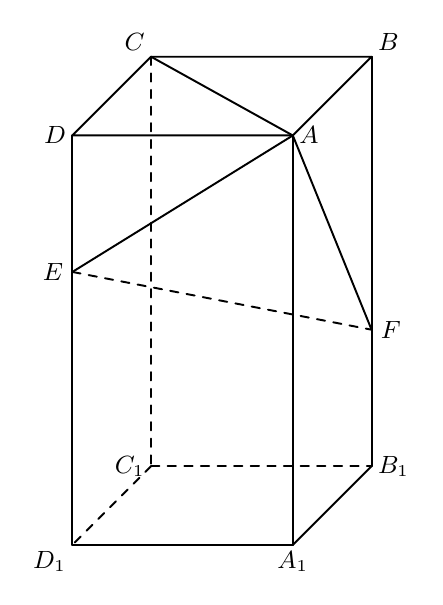
\begin{tikzpicture}[line width=0.7pt, font=\small,
  x=1cm, y=1cm, line cap=round, line join=round]

  % 顶点
  \coordinate (D)  at (0,5.20);
  \coordinate (A)  at (2.80,5.20);
  \coordinate (C)  at (1.00,6.20);
  \coordinate (B)  at (3.80,6.20);
  \coordinate (D1) at (0,0);
  \coordinate (A1) at (2.80,0);
  \coordinate (C1) at (1.00,1.00);
  \coordinate (B1) at (3.80,1.00);

  % E、F 按定比精确取点
  \coordinate (E) at (0,3.4667);
  \coordinate (F) at (3.80,2.7333);

  % 上底面
  \draw (D) -- (A) -- (B) -- (C) -- cycle;

  % 可见棱
  \draw (D) -- (D1);
  \draw (A) -- (A1);
  \draw (B) -- (B1);
  \draw (D1) -- (A1);
  \draw (A1) -- (B1);

  % 题设线段
  \draw (A) -- (C);
  \draw (A) -- (E);
  \draw (A) -- (F);

  % 被遮挡的棱与体内线段
  \draw[dashed] (C) -- (C1);
  \draw[dashed] (C1) -- (D1);
  \draw[dashed] (C1) -- (B1);
  \draw[dashed] (E) -- (F);

  % 顶点标注
  \node[above left,  inner sep=2pt] at (C)  {$C$};
  \node[above right, inner sep=2pt] at (B)  {$B$};
  \node[left,        inner sep=2pt] at (D)  {$D$};
  \node[right,       inner sep=2pt] at (A)  {$A$};
  \node[left,        inner sep=3pt] at (E)  {$E$};
  \node[right,       inner sep=3pt] at (F)  {$F$};
  \node[below left,  inner sep=2pt] at (D1) {$D_1$};
  \node[below,       inner sep=2pt] at (A1) {$A_1$};
  \node[left,        inner sep=2pt] at (C1) {$C_1$};
  \node[right,       inner sep=2pt] at (B1) {$B_1$};
\end{tikzpicture}
\end{center}
\nopagebreak[4]
\Needspace{4\baselineskip}
\textbf{解析}
\Needspace{5\baselineskip}
记
\nopagebreak[4]
\[\overrightarrow{AB}=\boldsymbol v,\qquad \overrightarrow{AD}=\boldsymbol u,\qquad \overrightarrow{AA_1}=\boldsymbol w .\]
由长方体知 $\boldsymbol u$，$\boldsymbol v$，$\boldsymbol w$ 两两垂直，$|\boldsymbol v|=AB$，$|\boldsymbol u|=AD=BC$。
\Needspace{5\baselineskip}
$E$ 在 $DD_1$ 上且 $2DE=ED_1$，即 $DE=\dfrac13DD_1$，而 $\overrightarrow{DD_1}=-\boldsymbol w$，故
\nopagebreak[4]
\[\overrightarrow{AE}=\overrightarrow{AD}+\overrightarrow{DE}=\boldsymbol u-\frac13\boldsymbol w .\]
\Needspace{5\baselineskip}
$F$ 在 $BB_1$ 上且 $BF=2FB_1$，即 $BF=\dfrac23BB_1$，而 $\overrightarrow{BB_1}=-\boldsymbol w$，故
\nopagebreak[4]
\[\overrightarrow{AF}=\overrightarrow{AB}+\overrightarrow{BF}=\boldsymbol v-\frac23\boldsymbol w .\]
\gksubpart{（1）}
\Needspace{5\baselineskip}
两式相减：
\nopagebreak[4]
\[\overrightarrow{EF}=\overrightarrow{AF}-\overrightarrow{AE}=\boldsymbol v-\boldsymbol u-\frac13\boldsymbol w .\]
\Needspace{5\baselineskip}
又 $\overrightarrow{AC}=\overrightarrow{AB}+\overrightarrow{BC}=\boldsymbol v+\boldsymbol u$，于是
\nopagebreak[4]
\[\overrightarrow{EF}\cdot\overrightarrow{AC}=\left(\boldsymbol v-\boldsymbol u-\frac13\boldsymbol w\right)\cdot(\boldsymbol v+\boldsymbol u)=|\boldsymbol v|^2-|\boldsymbol u|^2-\frac13\boldsymbol w\cdot(\boldsymbol v+\boldsymbol u) .\]
\Needspace{5\baselineskip}
因 $\boldsymbol w\perp\boldsymbol v$，$\boldsymbol w\perp\boldsymbol u$，末项为零；又 $AB=BC$ 时 $|\boldsymbol v|=|\boldsymbol u|$，故
\nopagebreak[4]
\[\overrightarrow{EF}\cdot\overrightarrow{AC}=AB^2-BC^2=0,\]
即 $EF\perp AC$。
\gksubpart{（2）}
\Needspace{5\baselineskip}
把上面两式相加：
\nopagebreak[4]
\[\overrightarrow{AE}+\overrightarrow{AF}=\left(\boldsymbol u-\frac13\boldsymbol w\right)+\left(\boldsymbol v-\frac23\boldsymbol w\right)=\boldsymbol u+\boldsymbol v-\boldsymbol w .\]
\Needspace{5\baselineskip}
而
\nopagebreak[4]
\[\overrightarrow{AC_1}=\overrightarrow{AC}+\overrightarrow{CC_1}=(\boldsymbol u+\boldsymbol v)-\boldsymbol w,\]
\Needspace{5\baselineskip}
故
\nopagebreak[4]
\[\overrightarrow{AC_1}=\overrightarrow{AE}+\overrightarrow{AF}.\]
这说明 $\overrightarrow{AC_1}$ 是平面 $AEF$ 内两个不共线向量 $\overrightarrow{AE}$，$\overrightarrow{AF}$ 的线性组合，即 $C_1$ 在平面 $AEF$ 内。

\gkanswer{答案（1）：证明。向量法得 $\overrightarrow{EF}\cdot\overrightarrow{AC}=AB^2-BC^2=0$，故 $EF\perp AC$。}

\gkanswer{答案（2）：证明。由 $\overrightarrow{AC_1}=\overrightarrow{AE}+\overrightarrow{AF}$ 得 $C_1$ 在平面 $AEF$ 内。}

\end{answer}
\begin{answer}
\gksolhead{20}{}

\textbf{题目}：

已知函数 $f(x)=x^3-kx+k^2$。
（1） 讨论 $f(x)$ 的单调性；
（2） 若 $f(x)$ 有三个零点，求 $k$ 的取值范围。

\Needspace{4\baselineskip}
\textbf{解析}
\gksubpart{（1）}
\nopagebreak[4]
\[f'(x)=3x^2-k .\]
若 $k\leqslant0$，则 $f'(x)\geqslant0$ 对一切 $x$ 成立（$k=0$ 时仅 $x=0$ 处为零），故 $f(x)$ 在 $\mathbf R$ 上单调递增。
\Needspace{5\baselineskip}
若 $k>0$，则 $f'(x)=0$ 的两根为
\nopagebreak[4]
\[x_1=-\sqrt{\frac k3},\qquad x_2=\sqrt{\frac k3},\]
\Needspace{5\baselineskip}
且 $f'(x)=3(x-x_1)(x-x_2)$ 的符号为：$x<x_1$ 时正，$x_1<x<x_2$ 时负，$x>x_2$ 时正。故 $f(x)$ 在
\nopagebreak[4]
\[\left(-\infty,-\sqrt{\frac k3}\right),\quad \left(\sqrt{\frac k3},+\infty\right)\]
\Needspace{5\baselineskip}
上单调递增，在
\nopagebreak[4]
\[\left(-\sqrt{\frac k3},\sqrt{\frac k3}\right)\]
上单调递减。
\gksubpart{（2）}
\Needspace{5\baselineskip}
若 $f$ 有三个零点，必须 $k>0$（$k\leqslant0$ 时 $f$ 严格单调，至多一个零点）。此时 $x_1$ 为极大值点，$x_2$ 为极小值点。计算极值：由 $x_i^2=\dfrac k3$ 得 $x_i^3=\dfrac k3x_i$，故
\nopagebreak[4]
\[f(x_i)=x_i^3-kx_i+k^2=\frac k3x_i-kx_i+k^2=k^2-\frac{2k}3x_i .\]
\Needspace{5\baselineskip}
于是
\nopagebreak[4]
\[f(x_1)=k^2+\frac{2k}3\sqrt{\frac k3}>0,\qquad f(x_2)=k^2-\frac{2k}3\sqrt{\frac k3} .\]
\Needspace{5\baselineskip}
极大值恒正；要有三个零点，只需极小值为负：
\nopagebreak[4]
\[k^2-\frac{2k}3\sqrt{\frac k3}<0\ \Longrightarrow\ k<\frac23\sqrt{\frac k3},\]
\Needspace{5\baselineskip}
两边平方（$k>0$）：
\nopagebreak[4]
\[k^2<\frac49\cdot\frac k3=\frac{4k}{27}\ \Longrightarrow\ k<\frac4{27} .\]
此时由单调性：$f$ 在 $\left(-\infty,x_1\right)$ 上从 $-\infty$ 增到 $f(x_1)>0$，在 $(x_1,x_2)$ 上从正降到 $f(x_2)<0$，在 $(x_2,+\infty)$ 上从负增到 $+\infty$，三个区间各恰有一个零点，共三个。
\Needspace{5\baselineskip}
故 $k$ 的取值范围是
\nopagebreak[4]
\[\left(0,\frac4{27}\right).\]

\gkanswer{答案（1）：$k\leqslant0$ 时在 $\mathbf R$ 上单调递增；$k>0$ 时在 $\left(-\infty,-\sqrt{\dfrac k3}\right)$ 与 $\left(\sqrt{\dfrac k3},+\infty\right)$ 上单调递增，在 $\left(-\sqrt{\dfrac k3},\sqrt{\dfrac k3}\right)$ 上单调递减。}

\gkanswer{答案（2）：$\left(0,\dfrac4{27}\right)$。极大值 $k^2+\dfrac23k\sqrt{\dfrac k3}>0$ 恒成立，极小值 $k^2-\dfrac23k\sqrt{\dfrac k3}<0$ 等价于 $k<\dfrac4{27}$。}

\end{answer}
\begin{answer}
\gksolhead{21}{}

\textbf{题目}：

已知椭圆 $C:\dfrac{x^2}{25}+\dfrac{y^2}{m^2}=1$（$0<m<5$）的离心率为 $\dfrac{\sqrt{15}}4$，$A$，$B$ 分别为 $C$ 的左、右顶点。
（1） 求 $C$ 的方程；
（2） 若点 $P$ 在 $C$ 上，点 $Q$ 在直线 $x=6$ 上，且 $|BP|=|BQ|$，$BP\perp BQ$，求 $\triangle APQ$ 的面积。

\Needspace{4\baselineskip}
\textbf{解析}
\gksubpart{（1）}
\Needspace{5\baselineskip}
由 $C:\dfrac{x^2}{25}+\dfrac{y^2}{m^2}=1$ 知 $a=5$，$b=m$，$c^2=25-m^2$。离心率
\nopagebreak[4]
\[e^2=\frac{c^2}{a^2}=\frac{25-m^2}{25}=\left(\frac{\sqrt{15}}4\right)^2=\frac{15}{16},\]
\Needspace{5\baselineskip}
故
\nopagebreak[4]
\[25-m^2=25\times\frac{15}{16}=\frac{375}{16}\ \Longrightarrow\ m^2=25-\frac{375}{16}=\frac{25}{16},\]
\Needspace{5\baselineskip}
与 $0<m<5$ 相符（$m=\dfrac54$）。所以
\nopagebreak[4]
\[C:\frac{x^2}{25}+\frac{16y^2}{25}=1 .\]
\gksubpart{（2）}
\Needspace{5\baselineskip}
由（1）$b^2=\dfrac{25}{16}$，椭圆即
\nopagebreak[4]
\[x^2+16y^2=25,\]
\Needspace{5\baselineskip}
左、右顶点为 $A(-5,0)$，$B(5,0)$。设 $Q(6,q)$，则
\nopagebreak[4]
\[\overrightarrow{BQ}=(1,q),\qquad |BQ|=\sqrt{1+q^2} .\]
\Needspace{5\baselineskip}
由 $BP\perp BQ$ 且 $|BP|=|BQ|$ 知 $\overrightarrow{BP}$ 是 $\overrightarrow{BQ}$ 绕 $B$ 旋转 $90^\circ$ 所得的向量，即
\nopagebreak[4]
\[\overrightarrow{BP}=(-q,1)\quad\text{\text{或}}\quad\overrightarrow{BP}=(q,-1).\]
\Needspace{5\baselineskip}
于是
\nopagebreak[4]
\[P(5-q,1)\quad\text{\text{或}}\quad P(5+q,-1).\]
\Needspace{5\baselineskip}
先看 $P(5-q,1)$：代入 $x^2+16y^2=25$ 得
\nopagebreak[4]
\[(5-q)^2+16=25\ \Longrightarrow\ (5-q)^2=9\ \Longrightarrow\ q=2\ \text{\text{或}}\ q=8,\]
对应 $P(3,1)$ 或 $P(-3,1)$。
\Needspace{5\baselineskip}
再看 $P(5+q,-1)$：同理
\nopagebreak[4]
\[(5+q)^2=9\ \Longrightarrow\ q=-2\ \text{\text{或}}\ q=-8,\]
对应 $P(3,-1)$ 或 $P(-3,-1)$。
\Needspace{5\baselineskip}
四种情形关于 $x$ 轴对称，面积相同，取 $P(3,1)$，$Q(6,2)$ 计算。此时
\nopagebreak[4]
\[\overrightarrow{AP}=(3+5,\ 1-0)=(8,1),\qquad \overrightarrow{AQ}=(6+5,\ 2-0)=(11,2),\]
\Needspace{5\baselineskip}
故
\nopagebreak[4]
\[S_{\triangle APQ}=\frac12\left|8\times2-1\times11\right|=\frac12\left|16-11\right|=\frac52 .\]
\Needspace{5\baselineskip}
逐一核对另三种情形：
\nopagebreak[4]
\[P(-3,1),Q(6,8):\ \frac12|2\times8-1\times11|=\frac52;\qquad P(3,-1),Q(6,-2):\ \frac12|8\times(-2)-(-1)\times11|=\frac52;\]
\nopagebreak[4]
\[P(-3,-1),Q(6,-8):\ \frac12|2\times(-8)-(-1)\times11|=\frac52 .\]
故 $\triangle APQ$ 的面积为 $\dfrac52$。

\gkanswer{答案（1）：$\dfrac{x^2}{25}+\dfrac{16y^2}{25}=1$。由 $e^2=\dfrac{25-m^2}{25}=\dfrac{15}{16}$ 得 $m^2=\dfrac{25}{16}$。}

\gkanswer{答案（2）：$\dfrac52$。设 $Q(6,q)$，由垂直且等长得 $P(5-q,1)$ 或 $P(5+q,-1)$，代回椭圆得 $q=\pm2$ 或 $q=\pm8$，四种情形的面积同为 $\dfrac52$。}

\end{answer}
\begin{answer}
\gksolhead{22}{【A】选修 4—4：坐标系与参数方程}

\textbf{题目}【A】（选修 4—4：坐标系与参数方程）：

在直角坐标系 $xOy$ 中，曲线 $C$ 的参数方程为 $\begin{cases}x=2-t-t^2,\\y=2-3t+t^2\end{cases}$（$t$ 为参数且 $t\neq1$），$C$ 与坐标轴交于 $A$，$B$ 两点。
（1） 求 $|AB|$；
（2） 以坐标原点为极点，$x$ 轴正半轴为极轴建立极坐标系，求直线 $AB$ 的极坐标方程。

\Needspace{4\baselineskip}
\textbf{解析}
\gksubpart{（1）}
\Needspace{5\baselineskip}
与 $x$ 轴的交点满足 $y=0$：
\nopagebreak[4]
\[2-3t+t^2=0\ \Longrightarrow\ (t-1)(t-2)=0\ \Longrightarrow\ t=1\ \text{\text{或}}\ t=2 .\]
因 $t\neq1$，取 $t=2$，得 $x=2-2-2^2=-4$，即交点 $(-4,0)$。
\Needspace{5\baselineskip}
与 $y$ 轴的交点满足 $x=0$：
\nopagebreak[4]
\[2-t-t^2=0\ \Longrightarrow\ (t-1)(t+2)=0\ \Longrightarrow\ t=1\ \text{\text{或}}\ t=-2 .\]
因 $t\neq1$，取 $t=-2$，得 $y=2-3\times(-2)+(-2)^2=2+6+4=12$，即交点 $(0,12)$。
\Needspace{5\baselineskip}
不妨记 $A(-4,0)$，$B(0,12)$，则
\nopagebreak[4]
\[|AB|=\sqrt{(0+4)^2+(12-0)^2}=\sqrt{16+144}=\sqrt{160}=4\sqrt{10} .\]
\gksubpart{（2）}
\Needspace{5\baselineskip}
由 $A(-4,0)$，$B(0,12)$ 得直线 $AB$ 的斜率为
\nopagebreak[4]
\[k=\frac{12-0}{0-(-4)}=3,\]
\Needspace{5\baselineskip}
故直角坐标方程为
\nopagebreak[4]
\[y=3(x+4),\quad\text{\text{即}}\quad 3x-y+12=0 .\]
\Needspace{5\baselineskip}
代入极坐标变换 $x=\rho\cos\theta$，$y=\rho\sin\theta$：
\nopagebreak[4]
\[3\rho\cos\theta-\rho\sin\theta+12=0,\]
\Needspace{5\baselineskip}
即
\nopagebreak[4]
\[\rho\left(\sin\theta-3\cos\theta\right)=12 .\]
这就是直线 $AB$ 的极坐标方程。

\gkanswer{答案（1）：$4\sqrt{10}$。令 $y=0$ 得 $t=2$、$A(-4,0)$，令 $x=0$ 得 $t=-2$、$B(0,12)$，故 $|AB|=\sqrt{16+144}=4\sqrt{10}$。}

\gkanswer{答案（2）：$3\rho\cos\theta-\rho\sin\theta+12=0$（即 $\rho(\sin\theta-3\cos\theta)=12$）。直线 $AB$ 的直角坐标方程为 $3x-y+12=0$，代入 $x=\rho\cos\theta$，$y=\rho\sin\theta$ 即得。}

\end{answer}
\begin{answer}
\gksolhead{23}{【B】选修 4—5：不等式选讲}

\textbf{题目}【B】（选修 4—5：不等式选讲）：

设 $a$，$b$，$c\in\mathbf R$，$a+b+c=0$，$abc=1$。
（1） 证明：$ab+bc+ca<0$；
（2） 用 $\max\{a,b,c\}$ 表示 $a$，$b$，$c$ 中的最大值，证明：$\max\{a,b,c\}\geqslant\sqrt[3]{4}$。

\Needspace{4\baselineskip}
\textbf{解析}
\gksubpart{（1）}
\Needspace{5\baselineskip}
由 $a+b+c=0$ 两边平方：
\nopagebreak[4]
\[0=(a+b+c)^2=a^2+b^2+c^2+2(ab+bc+ca),\]
\Needspace{5\baselineskip}
故
\nopagebreak[4]
\[ab+bc+ca=-\frac{a^2+b^2+c^2}2 .\]
\Needspace{5\baselineskip}
又 $abc=1$ 说明 $a$，$b$，$c$ 都不为 $0$，从而 $a^2+b^2+c^2>0$，于是
\nopagebreak[4]
\[ab+bc+ca=-\frac{a^2+b^2+c^2}2<0 .\]
\gksubpart{（2）}
设 $a=\max\{a,b,c\}$。
\Needspace{5\baselineskip}
先确定符号：由 $abc=1>0$ 知三数全正或两负一正；若全正则 $a+b+c>0$，与 $a+b+c=0$ 矛盾。故三数中恰有一个为正、两个为负，而正数就是最大数，即
\nopagebreak[4]
\[a>0,\qquad b<0,\qquad c<0 .\]
\Needspace{5\baselineskip}
由韦达定理，$b$，$c$ 是方程
\nopagebreak[4]
\[t^2-(b+c)t+bc=t^2+at+\frac1a=0\]
\Needspace{5\baselineskip}
的两个实根（这里用了 $b+c=-a$ 与 $bc=\dfrac{abc}a=\dfrac1a$）。因 $b$，$c$ 为实数，判别式非负：
\nopagebreak[4]
\[\Delta=a^2-\frac4a\geqslant0\ \Longrightarrow\ a^3\geqslant4\ \Longrightarrow\ a\geqslant\sqrt[3]{4} .\]
\Needspace{5\baselineskip}
故
\nopagebreak[4]
\[\max\{a,b,c\}\geqslant\sqrt[3]{4} .\]
等号在 $b=c$ 时成立，此时 $b=c=-\dfrac a2$，$bc=\dfrac{a^2}4=\dfrac1a$，即 $a^3=4$。

\gkanswer{答案（1）：证明。由 $(a+b+c)^2=0$ 得 $ab+bc+ca=-\dfrac{a^2+b^2+c^2}2$，而 $abc=1$ 保证 $a^2+b^2+c^2>0$，故 $ab+bc+ca<0$。}

\gkanswer{答案（2）：证明。最大值 $a>0$，$b$，$c$ 为 $t^2+at+\dfrac1a=0$ 的两实根，判别式 $a^2-\dfrac4a\geqslant0$，故 $a^3\geqslant4$，即 $a\geqslant\sqrt[3]{4}$。}

\end{answer}